\documentclass[presentation]{beamer}

\usepackage{tikz}
\usetikzlibrary{positioning,calc}
\usetikzlibrary{shapes.geometric}
\usetikzlibrary{backgrounds}% only to show the bounding box
\usetikzlibrary{shapes,arrows}
\usepackage{pgf}
\usepackage{pgfplots}
\usepackage{pgfplotstable}
\usepackage{appendixnumberbeamer}
\usepackage{amsmath}
\DeclareMathOperator{\tr}{tr}
\date{28th March 2017}
\usetheme{firedrake}
\firedrakeset{progressbar=frametitle}

\renewcommand{\vec}[1]{\ensuremath{\boldsymbol{#1}}}
\newcommand{\ddt}[1]{\frac{\partial #1}{\partial t}}
\newcommand{\zhat}{\hat{\vec{z}}}
\newcommand{\W}{\ensuremath{\mathbb{W}}}

\newcommand{\inner}[1]{\left\langle #1 \right \rangle}

\newcommand{\KSP}[2]{\ensuremath{\mathcal{K}\left(#1, \mathbb{#2}\right)}}
\newcommand{\ksp}[1]{\KSP{#1}{#1}}

\newcommand{\highlight}[1]{\colorbox{red!20}{\color{black} #1}}
\newcommand{\arxivlink}[2]{%
  \href{http://www.arxiv.org/abs/#1}%
  {{\small\texttt{arXiv:\,#1\,[#2]}}}%
}
\newcommand{\doilink}[1]{%
  \href{http://dx.doi.org/#1}%
  {{\small\texttt{doi:\,#1}{}}}%
}

\author{Lawrence Mitchell\inst{1,*}}
\institute{
\inst{1}Departments of Computing and Mathematics, Imperial College
London

\inst{*}\texttt{lawrence.mitchell@imperial.ac.uk}
}

\graphicspath{{./\jobname.figures/}}

\usepackage[url=false,
            doi=true,
            isbn=false,
            style=authoryear,
            firstinits=true,
            uniquename=init,
            backend=biber]{biblatex}

\setbeamertemplate{bibliography item}{}

\renewcommand{\bibfont}{\footnotesize}
\addbibresource{references.bib}

\setlength{\bibitemsep}{1ex}
\setlength{\fboxsep}{1pt}

\renewbibmacro{in:}{}
\DeclareFieldFormat[article]{volume}{\textbf{#1}}
\DeclareFieldFormat{doi}{%
  doi\addcolon%
  {\scriptsize\ifhyperref{\href{http://dx.doi.org/#1}{\nolinkurl{#1}}}
    {\nolinkurl{#1}}}}
\AtEveryBibitem{%
\clearfield{pages}%
\clearfield{issue}%
\clearfield{number}%
}

\usepackage{minted}
\RecustomVerbatimEnvironment{Verbatim}{BVerbatim}{}

\title{Firedrake: symbolic numerical computing}
\begin{document}

\maketitle

\setbeamertemplate{background}{}
\setbeamercolor{footline}{
  use=normal text,
  fg=normal text.fg,
}

% \begin{abstract}
%   One of the great and enduring successes of numerical computing is
%   the capturing of mathematical abstractions in software.  This allows
%   the programmer to express the intent of their code, without
%   specifying its low-level implementation.  We then automate the
%   synthesis of efficient code by using (or writing) compilers.

%   In the context of solving numerical PDEs, the finite element method
%   is particularly amenable to this approach.  For many problems, the
%   choice of discretisation completely specifies the mathematical
%   intent.  A symbolic description of the PDE can then be manipulated
%   by a domain-specific compiler to produce a high-performance
%   implementation.  I this talk, I present Firedrake
%   (www.firedrakeproject.org), a concrete realisation of this idea.  I
%   will discuss how capturing and exploiting symbolic structure in
%   numerical software greatly simplifies model development while
%   simultaneously permitting the synthesis of a high performance
%   implementation.  I will illustrate with examples from high-order
%   finite element methods, and block preconditioning of multiphysics
%   problems.
% \end{abstract}

\section{Introduction}
\begin{frame}
  \frametitle{Finite element crash course}
  \begin{align*}
    F(u) &= 0 \text{ in $\Omega$}\\
    u &= g \text{ on $\Gamma_1$}\\
    \frac{\partial u}{\partial n} &= h \text{ on $\Gamma_2$}
  \end{align*}
  Seek \emph{weak} solution in some space of functions $V(\Omega)$.

  Now we need to solve the (infinite dimensional) problem, find $u\in V$ s.t.
  \begin{equation*}
    \int_\Omega \!F(u) v\, \text{d}x = 0 \quad \forall\, v \in V
  \end{equation*}
\end{frame}
\begin{frame}
  \frametitle{Finite element crash course}
  Choose finite dimensional $V_h \subset V$, and seek a solution in
  that subspace: find $u_h \in V_h$ s.t.
  \begin{equation*}
    \int_\Omega \!F(u_h) v_h\, \text{d}x = 0 \quad \forall\, v_h \in V_h
  \end{equation*}
\end{frame}
\begin{frame}
  \frametitle{Finite element crash course}
  \begin{overprint}
    \only<1>{Divide domain $\Omega$\dots
    \begin{center}
      \begin{tikzpicture}
        \draw[very thick, line cap=rect] (0,0) -- (5, 0) (0, 0) arc
        (180:360:2.5);
      \end{tikzpicture}
    \end{center}}
  \only<2>{\dots{}into triangulation $\mathcal{T}$\dots
    \begin{center}
        \begin{tikzpicture}
          \path (0,0) arc[radius=2.5, start angle=180, end angle=360]
          node[name=E,pos=0,swap] {} node[name=F,pos=0.25,swap] {}
          node[name=G,pos=0.5,swap] {} node[name=H,pos=0.82,swap] {}
          node[name=I,pos=1,swap] {}; \node (A) at (2.5, 0) {}; \node
          (B) at (1.4, -0.7) {}; \node (C) at (3.4, -1.2) {}; \node
          (D) at (1.8, -1.5) {};

          \draw[color=black, very thick, line cap=butt, line
          join=round] (E.center) -- (A.center) -- (I.center) --
          (H.center) -- (G.center) -- (F.center) -- (E.center) --
          cycle; \draw[color=black, very thick, line cap=butt, line
          join=round] (E.center) -- (B.center) -- (D.center) --
          (F.center) -- (B.center); \draw[color=black, very thick,
          line cap=butt, line join=round] (G.center) -- (D.center) --
          (C.center) -- (G.center); \draw[color=black, very thick,
          line cap=butt, line join=round] (B.center) -- (A.center) --
          (C.center) -- (B.center); \draw[color=black, very thick,
          line cap=butt, line join=round] (H.center) -- (C.center) --
          (I.center);
        \end{tikzpicture}
    \end{center}
  }
  \only<3>{\dots{}and choose basis with finite support.
    \begin{center}
        \begin{tikzpicture}
          \path (0,0) arc[radius=2.5, start angle=180, end angle=360]
          node[name=E,pos=0,swap] {} node[name=F,pos=0.25,swap] {}
          node[name=G,pos=0.5,swap] {} node[name=H,pos=0.82,swap] {}
          node[name=I,pos=1,swap] {}; \node (A) at (2.5, 0) {}; \node
          (B) at (1.4, -0.7) {}; \node (C) at (3.4, -1.2) {}; \node
          (D) at (1.8, -1.5) {};

        \path[fill=gray!50] (E.center) -- (A.center) -- (B.center) --
        (F.center) --cycle;
          \draw[color=black, very thick, line cap=butt, line
          join=round] (E.center) -- (A.center) -- (I.center) --
          (H.center) -- (G.center) -- (F.center) -- (E.center) --
          cycle; \draw[color=black, very thick, line cap=butt, line
          join=round] (E.center) -- (B.center) -- (D.center) --
          (F.center) -- (B.center); \draw[color=black, very thick,
          line cap=butt, line join=round] (G.center) -- (D.center) --
          (C.center) -- (G.center); \draw[color=black, very thick,
          line cap=butt, line join=round] (B.center) -- (A.center) --
          (C.center) -- (B.center); \draw[color=black, very thick,
          line cap=butt, line join=round] (H.center) -- (C.center) --
          (I.center);
        \end{tikzpicture}
      \end{center}
      }
  \end{overprint}
\end{frame}

\begin{frame}
  \frametitle{Finite element crash course}
  Integrals become sum over element integrals
  \begin{equation*}
    \int_\Omega\! F(u_h) v_h \, \text{d}x =
    \sum_{e \in \mathcal{T}} \int_e\! F(u_h)v_h\, \text{d}x
  \end{equation*}

  (Usually) perform element integrals with numerical quadrature
  \begin{equation*}
    \int_e F(u_h)v_h\,\text{d}x = \sum_q w_q F(u_h(q)) v_h(q)\,\text{d}x
  \end{equation*}

  Replace $u_h(q), v_h(q)$ with expansion in finite element basis
  \begin{align*}
    u_h(q) &= \sum_i u_h^i \phi_i(q)\\
    v_h(q) &= \phi_j(q)\\
  \end{align*}
\end{frame}

\begin{frame}
  \frametitle{Abstractly}
  \begin{itemize}
  \item Mathematics says ``here is the integral to compute on each
    element, do that everywhere''
  \item Doesn't specify \emph{how} to compute the integral
  \item Doesn't specify \emph{how} to gather the element contributions
  \end{itemize}
\end{frame}

\section{Compilers for finite elements}

\begin{frame}
  \frametitle{Specifying element integrals}

  Traditional software libraries for finite element computations give you
  \begin{itemize}
  \item methods for computing numerical quadrature
  \item methods to evaluate basis functions at quadrature points
  \item methods to evaluate fields at quadrature points
  \item methods to compute geometric transformations
  \end{itemize}
\end{frame}
\begin{frame}[fragile]
  \frametitle{Specifying element integrals}
  Some typical hand-written code.

  \begin{center}
\begin{minted}[fontsize=\tiny]{cpp}
template<typename EG, typename LFSU, typename X, typename LFSV, typename M>
void jacobian_volume(const EG& eg, const LFSU& lfsu, const X& x,
                     const LFSV& lfsv, M& mat) const {
  const auto geo = eg.geometry();
  const auto S = geo.jacobianInverseTransposed(qp);
  RF factor = weight*geo.integrationElement(qp);
  double grad[dim][n] = {{0.0}};
  for (int i=0; i<dim; i++)
    for (int k=0; k<dim; k++)
      for (int j=0; j<n; j++)
        grad[i][j] += S[i][k] * gradhat[k][j];
  double A[n][n] = {{0.0}};
  for (int i=0; i<n; i++)
    for (int k=0; k<dim; k++)
      for (int j=0; j<n; j++)
        A[i][j] += grad[k][i]*grad[k][j];
  for (int i=0; i<n; i++)
    for (int j=0; j<n; j++)
      mat.accumulate(lfsu,i,lfsu,j,A[i][j]*factor);
}
\end{minted}
  \end{center}
  \begin{uncoverenv}<2>
    \begin{equation*}
      \int_\Omega \nabla u \cdot \nabla v\,\text{d}x
    \end{equation*}
  \end{uncoverenv}
\end{frame}

\begin{frame}
  \frametitle{Replacing humans with computers}
  \begin{block}{Assertion}
    Once we pick the discretisation, writing the element integral is mechanical.
  \end{block}
  \begin{corollary}
    Computers are good at mechanical things, why don't we get the
    computer to write the element integral?
  \end{corollary}
\end{frame}

\begin{frame}
  \frametitle{Firedrake}
  An automated finite element system.

  \begin{center}
    \url{www.firedrakeproject.org}\\
    \cite{Rathgeber:2016} \arxivlink{1501.01809}{cs.MS}
  \end{center}

  \begin{overlayarea}{\textwidth}{0.6\textheight}
    \only<1>{%
      \begin{block}{Development team}
        \begin{itemize}
        \item[IC] Thomas Gibson, David A.~Ham, Mikl\'os Homolya,
          Lawrence Mitchell, {\color{black!50}Fabio Luporini},
          Tianjiao Sun, Paul H.~J.~Kelly
        \item[\color{black!75}Baylor] {\color{black!75}Robert
            C. Kirby}
        \item[\color{black!75}Bath] {\color{black!75}Andrew
            T.~T.~McRae}
        \item[\color{black!25}ECMWF] {\color{black!25}Florian
            Rathgeber}
        \item[\color{black!15}IBM] {\color{black!15}Gheorghe-Teodor
            Bercea}
        \end{itemize}
      \end{block}
    }%
    \only<2>{%
      \begin{block}{Users at}
        Imperial, Bath, Leeds, Kiel, Rice, Houston, Oregon Health \&
        Science, Exeter, ETH, Waterloo, Minnesota, Baylor \dots
      \end{block}
    }
  \end{overlayarea}
\end{frame}

\begin{frame}
  \frametitle{Exploiting abstractions}
  \begin{itemize}
  \item Firedrake builds on, and extends, embedded DSLs developed in
    the FEniCS project \url{www.fenicsproject.org}
  \item The \emph{Unified Form Language} \parencite{Alnaes:2014} to
    specify variational forms
  \item A symbolic problem description (generic) is woven together with
    problem-specific data, and executed by a runtime Python library
    that does JIT code compilation.
  \end{itemize}
\end{frame}

\begin{frame}
  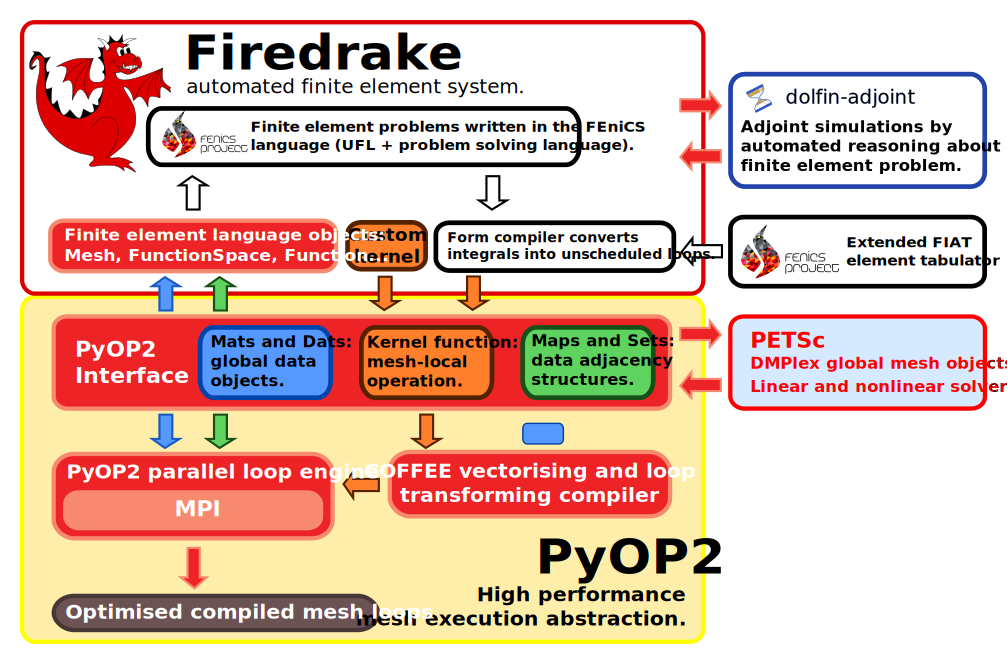
\includegraphics[width=\textwidth]{firedrake-stack}
\end{frame}

\begin{frame}[fragile]
  \frametitle{UFL: a DSL for variational problems}
  \begin{equation*}
    \int_\Omega \nabla u \cdot \nabla v\,\text{d}x
  \end{equation*}

\begin{minted}[fontsize=\scriptsize]{python}
V = FiniteElement("Lagrange", triangle, 1)
u = TrialFunction(V)
v = TestFunction(V)
a = dot(grad(u), grad(v))*dx
\end{minted}
\end{frame}

\begin{frame}[fragile]
  \frametitle{Not just toy models}
  \begin{columns}
    \begin{column}{0.4\textwidth}
      \begin{align*}
        \mathbf{F} &= \mathbf{I} + \nabla \mathbf{u}\\
        \mathbf{C} &= \mathbf{F}^T \mathbf{F}\\
        \mathbf{E} &= (\mathbf{C} - \mathbf{I}) / 2\\
        \Psi &= \frac{\lambda}{2}[\tr(\mathbf{E})]^2 + \mu \tr(\mathbf{E}^2)\\
        \mathbf{S} &= \frac{\partial \Psi}{\partial \mathbf{E}}\\
        \mathbf{P} &= \mathbf{F} \mathbf{S}\\
        r &= \int_\Omega \mathbf{P} : \nabla \mathbf{v} - \mathbf{b} \cdot \mathbf{v}\,\text{d}x\\
        a &= \lim_{\epsilon \to 0} \frac{r(\mathbf{u} + \epsilon \delta \mathbf{u}) - r(\mathbf{u})}{\epsilon}
      \end{align*}
    \end{column}
    \begin{column}{0.6\textwidth}
\begin{minted}[fontsize=\tiny]{python}
V = VectorElement("Lagrange", triangle, 2)
v = TestFunction(V)
du = TrialFunction(V) # Incremental displacement
u = Coefficient(V)    # Displacement
B = Coefficient(V)    # Body force per unit mass
I = Identity(V.cell().topological_dimension())
F = I+grad(u)  # Deformation gradient
C = F.T*F      # Right Cauchy-Green tensor
E = (C - I)/2
E = variable(E)
# Material constants
mu = Constant(triangle)
lmbda = Constant(triangle)
# Strain energy function (material model)
psi = lmbda/2*(tr(E)**2) + mu*tr(E*E)
S = diff(psi, E) # Second Piola-Kirchhoff stress tensor
P = F*S          # First Piola-Kirchoff stress tensor
# Variational problem
r = (inner(PK, grad(v)) - inner(B, v))*dx
a = derivative(r, u, du)
\end{minted}
    \end{column}
  \end{columns}  
\end{frame}

\begin{frame}[fragile]
  \frametitle{Mechanical translation}
  \begin{itemize}
  \item A \emph{form compiler} translates a symbolic description (UFL) into
    low-level (C/C++/...) code for performing an element integral.
  \end{itemize}
  \hspace{2em}
  \begin{uncoverenv}<2>
    \begin{columns}
      \begin{column}{0.5\textwidth}
\begin{minted}[fontsize=\tiny]{c}
void cell_integral(double A[3][3],
                   double coords[3][2]) {
  static const double t10[3] = {...};
  static const double t12[3] = {...};
  double t13[3];
  double t14[3];
  double t0 = (-1 * coords[0][1]);
  double t1 = (t0 + coords[1][1]);
  double t2 = (-1 * coords[0][0]);
  double t3 = (t2 + coords[1][0]);
  double t4 = (t0 + coords[2][1]);
  double t5 = (t2 + coords[2][0]);
  double t6 = ((t3 * t4) + (-1 * (t5 * t1)));
  double t7 = ((-1 * t1) / t6);
  double t8 = (t4 / t6);
  double t9 = (t3 / t6);
  double t11 = ((-1 * t5) / t6);
\end{minted}
      \end{column}
      \begin{column}{0.5\textwidth}
\begin{minted}[fontsize=\tiny]{c}
  for (int k0 = 0; k0 < 3; k0++) {
    t13[k0] = (t11 * t12[k0]) + (t9 * t10[k0]);
    t14[k0] = (t8 * t12[k0]) + (t7 * t10[k0]);
  }
  double t15 = (0.5 * fabs(t6));
  for (int j0 = 0; j0 < 3; j0++) {
    double t16 = ((t11 * t12[j0])
                  + (t9 * t10[j0]));
    double t17 = ((t8 * t12[j0])
                  + (t7 * t10[j0]));
    for (int k0 = 0; k0 < 3; k0++) {
      A[j0][k0] += t15 * ((t17 * t14[k0])
                          + (t16 * t13[k0]));
    }
  }
}
\end{minted}
      \end{column}
    \end{columns}
  \end{uncoverenv}
\end{frame}

\begin{frame}[fragile,plain]
  \begin{columns}
    \begin{column}{0.5\textwidth}
\begin{minted}[fontsize=\fontsize{4.3}{4.3}\selectfont]{c}
void cell_integral(double A[12][12], double coords[3][2],
                   double w_0[6][2], double w_1[1],
                   double w_2[2]) {
  static const double t0[2][2] = {...};
  static const double t9[6] = {...};
  static const double t15[6][6] = {...};
  static const double t16[6][6] = {...};
  double t1 = (-1 * coords[0][0]);
  double t2 = (t1 + coords[1][0]);
  double t3 = (-1 * coords[0][1]);
  double t4 = (t3 + coords[2][1]);
  double t5 = (t1 + coords[2][0]);
  double t6 = (t3 + coords[1][1]);
  double t7 = ((t2 * t4) + (-1 * (t5 * t6)));
  double t8 = fabs(t7);
  double t10 = (w_2[0] / 2);
  double t11 = (t2 / t7);
  double t12 = ((-1 * t5) / t7);
  double t13 = ((-1 * t6) / t7);
  double t14 = (t4 / t7);

  for (int ip = 0; ip < 6; ip++) {
    double t56[6][2] ;
    double t57[6][2] ;
    double t61[6][2] ;
    double t62[6][2] ;
    double t20 = 0.0;
    double t19 = 0.0;
    double t18 = 0.0;
    double t17 = 0.0;
    for (int i_0 = 0; i_0 < 6; i_0++) {
      t17 += t16[ip][i_0] * w_0[i_0][1];
      t18 += t15[ip][i_0] * w_0[i_0][1];
      t19 += t16[ip][i_0] * w_0[i_0][0];
      t20 += t15[ip][i_0] * w_0[i_0][0];
    }
    double t21 = (1 + ((t14 * t20) + (t13 * t19)));
    double t22 = ((t12 * t20) + (t11 * t19));
    double t23 = ((t14 * t18) + (t13 * t17));
    double t24 = (1 + ((t12 * t18) + (t11 * t17)));
    double t25 = (((t21 * t22) + (t23 * t24)) / 2);
    double t26 = ((t25 + t25) * w_1[0]);
    double t27 = ((-1 + ((t21 * t21) + (t23 * t23))) / 2);
    double t28 = ((-1 + ((t22 * t22) + (t24 * t24))) / 2);
    double t29 = ((2 * (t27 + t28)) * t10);
    double t30 = (t29 + ((t27 + t27) * w_1[0]));
    double t31 = (t29 + ((t28 + t28) * w_1[0]));
    double t32 = (((t22 * t21) + (t24 * t23)) / 2);
    double t33 = ((t32 + t32) * w_1[0]);
    for (int k0 = 0; k0 < 6; k0++) {
      for (int k1 = 0; k1 < 2; k1++) {
        double t34 = (t0[k1][1] * t15[ip][k0]);
        double t35 = (t0[k1][1] * t16[ip][k0]);
        double t36 = ((t14 * t34) + (t13 * t35));
\end{minted}
    \end{column}
    \begin{column}{0.5\textwidth}
\begin{minted}[fontsize=\fontsize{4.3}{4.3}\selectfont]{c}
        double t37 = (t0[k1][0] * t15[ip][k0]);
        double t38 = (t0[k1][0] * t16[ip][k0]);
        double t39 = ((t12 * t37) + (t11 * t38));
        double t40 = (t39 * t21);
        double t41 = ((t14 * t37) + (t13 * t38));
        double t42 = (t41 * t22);
        double t43 = ((t12 * t34) + (t11 * t35));
        double t44 = (t43 * t23);
        double t45 = (t36 * t24);
        double t46 = (((t40 + t42) + (t44 + t45)) / 2);
        double t47 = ((t46 + t46) * w_1[0]);
        double t48 = (t41 * t21);
        double t49 = (t36 * t23);
        double t50 = (((t48 + t48) + (t49 + t49)) / 2);
        double t51 = (t39 * t22);
        double t52 = (t43 * t24);
        double t53 = (((t51 + t51) + (t52 + t52)) / 2);
        double t54 = ((2 * (t50 + t53)) * t10);
        double t55 = (t54 + ((t53 + t53) * w_1[0]));
        t56[k0][k1] = ((t36 * t33) + (t47 * t23))
                       + ((t43 * t31) + (t55 * t24));
        t57[k0][k1] = ((t41 * t33) + (t47 * t21))
                       + ((t39 * t31) + (t55 * t22));
        double t58 = (t54 + ((t50 + t50) * w_1[0]));
        double t59 = (((t42 + t40) + (t45 + t44)) / 2);
        double t60 = ((t59 + t59) * w_1[0]);
        t61[k0][k1] = ((t36 * t30) + (t58 * t23))
                       + ((t43 * t26) + (t60 * t24));
        t62[k0][k1] = ((t41 * t30) + (t58 * t21))
                       + ((t39 * t26) + (t60 * t22));
      }
    }
    double t63 = (t9[ip] * t8);
    for (int j0 = 0; j0 < 6; j0++) {
      for (int j1 = 0; j1 < 2; j1++) {
        double t64 = (t0[j1][1] * t15[ip][j0]);
        double t65 = (t0[j1][1] * t16[ip][j0]);
        double t66 = ((t12 * t64) + (t11 * t65));
        double t67 = (t0[j1][0] * t15[ip][j0]);
        double t68 = (t0[j1][0] * t16[ip][j0]);
        double t69 = ((t12 * t67) + (t11 * t68));
        double t70 = ((t14 * t64) + (t13 * t65));
        double t71 = ((t14 * t67) + (t13 * t68));
        for (int k0 = 0; k0 < 6; k0++) {
          for (int k1 = 0; k1 < 2; k1++) {
            A[(j0 * 2) + j1][(k0 * 2) + k1] += t63 *
                (((t62[k0][k1] * t71) + (t61[k0][k1] * t70))
                 + ((t57[k0][k1] * t69) + (t56[k0][k1] * t66)));
          }
        }
      }
    }
  }
}
\end{minted}
    \end{column}
  \end{columns}
\end{frame}

\begin{frame}[fragile]
  \frametitle{Optimisation of finite element kernels}
  
  \begin{problem}<+->
    Modern optimising compilers do a bad job on finite element
    kernels.
  \end{problem}
  \begin{exampleblock}<+->{Code motion (or not?)}
\begin{minted}[fontsize=\scriptsize]{c}
for (i = 0; i < L; i++ )
   for (j = 0; j < M; j++)
      for (k = 0; k < N; k++)
         A[j][k] += f(i, j)*g(i, k)
\end{minted}
  \end{exampleblock}
  \begin{corollary}<+->
    We need to spoon-feed the compiler already optimised code.
  \end{corollary}
\end{frame}

\begin{frame}
  \frametitle{Automating expertise}
  \begin{itemize}
  \item For a given kernel, can optimise by hand
  \item But this approach doesn't scale
  \item and the best strategy is problem-dependent.
  \item code generation allows us to package expertise, and provide it
    to everyone
  \end{itemize}
\end{frame}

\begin{frame}
  \frametitle{Different optimisations}
\begin{block}{Vectorisation}
  Align and pad data structures, then use intrinsics or rely on
  compiler. Generic to all kernels.

  \cite{Luporini:2015} \doilink{10.1145/2687415}
\end{block}

\begin{block}{Flop reduction}
  Exploit \emph{linearity} in test functions to perform factorisation,
  code motion and CSE.  Generic to all kernels.

  \cite{Luporini:2017} \arxivlink{1604.05872}{cs.MS}
\end{block}

\begin{block}{Sum factorisation}
  Optimal complexity for high order, enabled by development of a new
  form compiler, TSFC.  Only with structured basis.

  \cite{Homolya:2017} \arxivlink{1705.03667}{cs.MS}.
\end{block}
\end{frame}
\begin{frame}
  \frametitle{Sum factorisation}
  \begin{itemize}
  \item Consider evaluating a field, defined by basis coefficients
    $f_i$ at quadrature points $q$.

  \begin{equation*}
    \mathcal{F}_q = \sum_i \phi_{i,q} f_i
  \end{equation*}

  \item This matrix-vector product requires $\mathcal{O}(|i||q|) =
    \mathcal{O}(p^{2d})$ operations for polynomial degree $p$ in $d$
    dimensions.
  \item This quickly becomes huge for large $p$.
\end{itemize}
\end{frame}

\begin{frame}
  \frametitle{Exploiting structure}
  On many elements, there is \emph{structure} in the basis functions:
  \begin{equation*}
    \phi_{i,q} := \phi_{(j,k),(p,r)} = \varphi_{j,p}\varphi_{k,r}
  \end{equation*}
  and so
  \begin{align*}
    \mathcal{F}_{(p,r)} &= \sum_{j,k} \phi_{(j,k),(p,r)} f_{j,k} \\
                        &= \sum_{j,k} \varphi_{j,p}\varphi_{k,r} f_{j,k} \\
                        &= \sum_j \varphi_{j,p} \sum_k \varphi_{k,r} f_{j,k}
  \end{align*}
\end{frame}

\begin{frame}
  \frametitle{Large computational savings}
  \begin{itemize}
  \item Performing this transformation provides for \emph{optimal
      complexity} evaluation of matrix-vector products.

    \begin{center}
      \begin{tabular}{c|c|c|c}
        Method    & Build operator        & MatVec                  & Mem refs
        \\
                  & (FLOPs)               & (FLOPs)                 & (bytes)               \\
        \hline
        Assembled & $\mathcal{O}(p^{3d})$ & $\mathcal{O}(p^{2d})$   & $\mathcal{O}(p^{2d})$ \\
        MF        & 0                     & $\mathcal{O}(p^{2d})$   & $\mathcal{O}(p^d)$    \\
        MF + SF   & 0                     & $\mathcal{O}(dp^{d+1})$ & $\mathcal{O}(p^d)$
      \end{tabular}
    \end{center}
    
  \item This is necessary if we want high-order methods to be competitive.
  \end{itemize}
  
\end{frame}

\begin{frame}[fragile]
  \frametitle{Automated sum factorisation}
  \begin{itemize}
  \item C and Fortran compilers do not perform these transformations
  \item But they are easy on a structured expression-DAG
  \end{itemize}

  \begin{tikzpicture}
    \begin{loglogaxis}[name=plot,
      small,
      title=FLOPs for hyperelastic model on single hexahedron,
      xlabel=Polynomial degree,
      ylabel=FLOPs,
      xtick={1,2,4,8,16,32},
      xticklabels={$1$,$2$,$4$,$8$,$16$,$32$},
      yminorticks=false,
      axis lines=left,
      log basis x=2,
      legend entries={TSFC ``vanilla'', TSFC ``spectral''},
      legend style={cells={anchor=east},
        legend pos=outer north east,
        draw=none},
      ]
      \pgfplotstableread[format=inline]{
degree flops
1 57991.0
2 898053.0
3 5695832.0
4 23385568.0
5 73395072.0
6 191831126.0
7 439133008.0
8 909180492.0
9 1739859128.0
10 3125082802.0
11 5328273576.0
12 8697298808.0
13 13680865552.0
14 20846372238.0
15 30899217632.0
16 4.47036e+10
17 6.33046e+10
18 8.79521e+10
19 1.20126e+11
20 1.61561e+11
21 2.1428e+11
22 2.80615e+11
23 3.63248e+11
24 4.65233e+11
25 5.90039e+11
26 7.41582e+11
27 9.24258e+11
28 1.14299e+12
29 1.40325e+12
30 1.71113e+12
31 2.07336e+12
32 2.49735e+12
}\vanilla;

       \pgfplotstableread[format=inline]{
degree flops
1 11320
2 70587
3 227308
4 540688
5 1.09416e+06
6 1.98419e+06
7 3.32309e+06
8 5.23901e+06
9 7.87593e+06
10 1.13937e+07
11 1.59679e+07
12 2.17902e+07
13 2.90678e+07
14 3.8024e+07
15 4.88977e+07
16 6.19439e+07
17 7.74332e+07
18 9.56522e+07
19 1.16903e+08
20 1.41505e+08
21 1.69791e+08
22 2.02111e+08
23 2.38831e+08
24 2.80332e+08
25 3.27013e+08
26 3.79286e+08
27 4.37581e+08
28 5.02342e+08
29 5.7403e+08
30 6.53122e+08
31 7.4011e+08
32 8.35503e+08
}\sumfact;

      \pgfplotstableset{create on use/vanilla/.style={create
          col/expr={1e4*pow(\thisrow{degree},6)}}}
      \pgfplotstableset{create on use/spectral/.style={create
          col/expr={5e2*pow(\thisrow{degree},4)}}}
  
      \addplot+[mark=none, color=black, line width=1.5pt] table [x=degree,y=flops] \vanilla;
      \addplot+[mark=none, color=black, dashed, line width=1.5pt] table [x=degree,y=flops] \sumfact;
      \addplot+[mark=none, color=black, dotted, line width=1pt] table
      [x=degree,y=vanilla] \vanilla
      coordinate [pos=0.67] (A);
      \node at (A) [anchor=south east] {$\mathcal{O}(p^6)$};
      \addplot+[mark=none, color=black, dotted, line width=1pt] table
      [x=degree,y=spectral] \vanilla
      coordinate [pos=0.67] (B);
      \node at (B) [anchor=north west] {$\mathcal{O}(p^4)$};
    \end{loglogaxis}
  \end{tikzpicture}
\end{frame}

\section{Synthesising complete simulations}

\begin{frame}
  \frametitle{Synthesising efficient simulation code}
  \begin{itemize}
  \item Why stop at just a compiler for the element integral?
  \item The full mathematical problem specifies both the elementary
    integral and also the problem specific data.
  \item Why not capture this in software too?
  \end{itemize}
\end{frame}

\begin{frame}[fragile]
  \frametitle{A full specification of a problem}
  \begin{columns}
    \begin{column}{0.47\framewidth}
      \begin{block}{Stationary Rayleigh-B\'enard convection}
        \begin{equation*}
          \begin{split}
            -\Delta u + u\cdot\nabla u + \nabla p +
            \frac{\text{Ra}}{\text{Pr}} \hat{g}T &= 0 \\
            \nabla \cdot u &= 0 \\
            - \frac{1}{\text{Pr}} \Delta T + u\cdot \nabla T &= 0
          \end{split}
        \end{equation*}
      \end{block}
    \end{column}
    \begin{column}{0.52\framewidth}
\begin{minted}[fontsize=\tiny,mathescape]{python}
from firedrake import *
mesh = Mesh(...)
V = VectorFunctionSpace(mesh, "CG", 2)
W = FunctionSpace(mesh, "CG", 1)
Q = FunctionSpace(mesh, "CG", 1)
Z = V * W * Q
upT = Function(Z)
u, p, T = split(upT)
v, q, S = TestFunctions(Z)
bcs = [...] # no-flow + temp gradient
nullspace = MixedVectorSpaceBasis(
   Z, [Z.sub(0), VectorSpaceBasis(constant=True), 
       Z.sub(2)])
F = (inner(grad(u), grad(v))
     + inner(dot(grad(u), u), v)
     - inner(p, div(v))
     + (Ra/Pr)*inner(T*g, v)
     + inner(div(u), q)
     + inner(dot(grad(T), u), S)
     + (1/Pr) * inner(grad(T), grad(S)))*dx

solve(F == 0, upT, bcs=bcs, nullspace=nullspace)
\end{minted}
    \end{column}
  \end{columns}
\end{frame}

\begin{frame}
  \frametitle{More than a pretty face}

  \begin{block}{Library usability}
    \begin{itemize}
    \item High-level language enables rapid model development
    \item Ease of experimentation
    \item Small model code base
    \end{itemize}
  \end{block}

  \begin{block}{Library development}
    \begin{itemize}
    \item Automation of complex optimisations
    \item Exploit expertise across disciplines
    \item Small library code base
    \end{itemize}
  \end{block}
\end{frame}

\begin{frame}[fragile]
  \frametitle{Automated manipulation of PDE solvers}
  \begin{itemize}
  \item With a high-level problem description language, we can write
    code that manipulates a PDE model.
  \end{itemize}

  \begin{block}{\url{www.dolfin-adjoint.org}}
    Automated derivation of the discrete adjoint from forward models
    written using FEniCS \emph{and Firedrake}.

\begin{minted}[fontsize=\scriptsize]{sh}
$ cloc dolfin-adjoint/
Language  files   blank   comment   code
Python       54    2322       937   7294
$ cloc dolfin-adjoint/compatibility.py
Python        1      38        11    140
\end{minted}
  \end{block}
\end{frame}

\begin{frame}
  \frametitle{Maintainability}
  \begin{columns}
    \begin{column}[t]{0.5\textwidth}
      \begin{block}{Core Firedrake}
        \begin{table}
          \centering
          \begin{tabular}{lc}
            Component & LOC   \\
            \hline
            Firedrake & 11500 \\
            PyOP2     & 6000  \\
            TSFC      & 3700  \\
            finat     & 800   \\
            \hline
            Total     & 22000
          \end{tabular}
        \end{table}
      \end{block}
    \end{column}
    \begin{column}[t]{0.5\textwidth}
      \begin{block}{Shared with FEniCS}
        \begin{table}
          \centering
          \begin{tabular}{lc}
            Component & LOC   \\
            \hline
            FIAT      & 4000  \\
            UFL       & 13000 \\
            \hline
            Total     & 17000
          \end{tabular}
        \end{table}        
      \end{block}
    \end{column}
  \end{columns}
\end{frame}

\begin{frame}
  \frametitle{Maintainable models}
  \begin{overlayarea}{\textwidth}{0.8\textheight}
    \begin{onlyenv}<1>
      \begin{block}{Thetis}
        \begin{center}
          \url{github.com/thetisproject/thetis}
        \end{center}
        \begin{itemize}
        \item 3D unstructured coastal ocean model written with
          Firedrake
        \item 6400 LOC
        \item 4-8x faster than previous code in group (same numerics)
        \end{itemize}
      \end{block}
    \end{onlyenv}
    \begin{onlyenv}<2>
      \begin{block}{Gusto}
        \begin{center}
          \url{www.firedrakeproject.org/gusto/}
        \end{center}
        \begin{itemize}
        \item 3D atmospheric dynamical core using compatible FE
        \item Implements Met Office ``Gung Ho'' numerics
        \item 1600 LOC
        \end{itemize}
      \end{block}
    \end{onlyenv}
  \end{overlayarea}
\end{frame}

\begin{frame}
  \frametitle{High performance}
  Fast prototyping is good, ``but I have to rewrite for performance''.

  \begin{uncoverenv}<2>
    \begin{itemize}
    \item Firedrake provides computational performance often >50\%
      achievable peak \parencite{Luporini:2015,Bercea:2016,Mitchell:2016}.
    \item Hero-coding necessary if you want the last 10-20\%
    \item ...but at what (person) cost?
    \end{itemize}
  \end{uncoverenv}
\end{frame}

\section{Solving implicit systems}

\begin{frame}
  \frametitle{So I can write down a residual}
  \begin{itemize}
  \item It is easy to write down complex implicit systems.
  \item the challenge is usually in solving them
  \item Firedrake provides access to PETSc for solving systems of
    algebraic equations
  \item ``Any'' algebraic solver you like, plus composition of block
    eliminations ``fieldsplit'' solvers.
  \end{itemize}
\end{frame}

\begin{frame}
  \frametitle{Coupled problems make this hard}
  \begin{itemize}
  \item Coupled problems are (typically) not amenable to black box solution
    methods.
  \item For large problems, often use approximate block factorisations.
  \item Many configuration options, may require problem-specific
    auxiliary operators.
  \item Important to capture the abstraction so that automated model
    manipulation is still possible.
  \end{itemize}
\end{frame}

\begin{frame}
  \frametitle{Block preconditioning}
  \begin{onlyenv}<1>
    \begin{itemize}
    \item Preconditioning for multi-variable problems is
      often based on block LU factorisations.
    \item Based on observation that
      \begin{equation*}
        T = \begin{bmatrix}
          A & 0 \\
          0 & - C A^{-1} B^T
        \end{bmatrix}^{-1}
        \begin{bmatrix}
          A & B^T \\
          C & 0
        \end{bmatrix}
      \end{equation*}
      has minimal polynomial $T(T - I)(T^2 - T - I) = 0$
      \parencite{Murphy:2000}.  
    \item With exact inverses, a Krylov method converges in at most 4 iterations.
    \end{itemize}
  \end{onlyenv}
  \begin{onlyenv}<2>
    \begin{itemize}
    \item Another approach is ``function space'' preconditioning
      \parencite{Kirby:2010,Mardal:2011,Malek:2014}.
    \item Removes mesh-dependence in iteration counts.
    \item e.g. Implicit timestepping for time-dependent Stokes
    \begin{equation*}
      \begin{bmatrix}
        \mathbb{I} - \Delta t \nabla^2 & -\nabla \\
        \nabla\cdot & 0
      \end{bmatrix}
    \end{equation*}
    Can be preconditioned by
    \begin{equation*}
      \begin{bmatrix}
        (\mathbb{I} - \Delta t\nabla^2)^{-1} & 0 \\
          0 & (-\nabla^2)^{-1} + \Delta t \mathbb{I}^{-1} \\
        \end{bmatrix}
      \end{equation*}
    \end{itemize}
  \end{onlyenv}
\end{frame}

\begin{frame}
  \frametitle{Extra challenges}
  \begin{itemize}
  \item Such preconditioners often require operators that do not
    appear in the original system
  \end{itemize}
  \begin{block}{Navier-Stokes}
    \begin{equation*}
      \begin{bmatrix}
        F & B^T\\
        C & 0 \\
      \end{bmatrix}
    \end{equation*}
    can be preconditioned using the pressure-convection-diffusion approximation
    \begin{equation*}
      \begin{bmatrix}
        F^{-1} & 0\\
        0 & L_p^{-1}F_p M_p^{-1}\\
      \end{bmatrix}
    \end{equation*}
    Where $L_p$ is a scalar Poisson operator, $M_p$ as mass matrix,
    and $F_p$ a scalar convection-diffusion operator.
  \end{block}
\end{frame}

\begin{frame}
  \frametitle{Reversing the one-way street}
  \begin{itemize}
  \item PETSc already provides a highly runtime-configurable library
    for \emph{algebraically} composing solvers \parencite{Brown:2012}.

  \item Firedrake makes it straightforward to build auxiliary
    operators.

  \item We combine these to allow simple development of complex
    preconditioners.
  \end{itemize}
\end{frame}

\begin{frame}
  \frametitle{Two new pieces}
 
  \begin{onlyenv}<1>
    \begin{block}{A new matrix type}
      A PETSc shell matrix that implements matrix-free actions using
      Firedrake, and contains the UFL of the bilinear form.
    \end{block}
    
    \begin{block}{Custom preconditioners}
      These matrices do not have entries, so we create custom
      preconditioners that can inspect the UFL and do the appropriate
      thing.
    \end{block}
  \end{onlyenv}
  \begin{onlyenv}<2>
    \begin{center}
      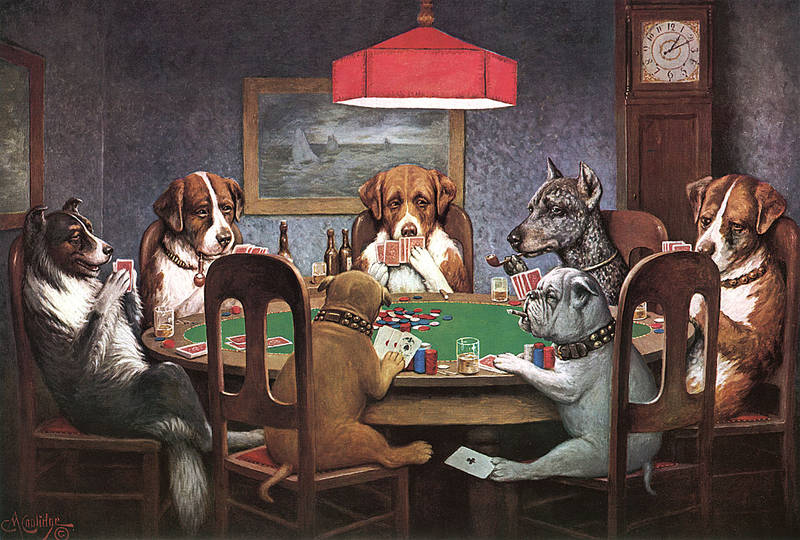
\includegraphics[width=0.8\textwidth]{underhand}
    \end{center}
  \end{onlyenv}
\end{frame}

\begin{frame}[fragile]
  \frametitle{PCD fits on a slide}
\begin{minted}[fontsize=\tiny,mathescape]{python}
class PCDPC(PCBase):
    def initialize(self, pc):
        _, P = pc.getOperators()
        ctx = P.getContext()
        appctx = ctx.appctx
        p, q = ctx.arguments()
        [...] # Handling of boundary conditions elided
        M_p = assemble(p*q*dx)
        L_p = assemble(inner(grad(p), grad(q))*dx
        M_ksp = KSP().create()
        M_ksp.setOperators(M_p)
        L_ksp = KSP().create()
        L_ksp.setOperators(L_p)
        [...] # Some boilerplate elided
        u0 = split(appctx["state"])[appctx["velocity_space"]]
        F_p = assemble(inner(grad(p), grad(q))*dx + inner(u0, grad(p))*q*dx)

    def apply(self, pc, x, y):
        # $y \leftarrow \KSP{L_p}{L} F_p \KSP{M_p}{M} x$
        a, b = self.workspace
        self.M_ksp.solve(x, a)
        self.F_p.mult(a, b)
        self.L_ksp.solve(b, y)
\end{minted}
\end{frame}

\begin{frame}
  \frametitle{Fast development}

  \begin{itemize}
  \item Firedrake's high-level syntax means building the auxiliary
    operators I need is straightforward
  \item The code automatically takes advantage of any improvements in
    the library (fast matrix actions, better vectorisation, etc\dots)
  \item Solvers are \emph{runtime configurable} without changing code
  \item Composes with nonlinear solvers that need linearisations, and
    PDE manipulation libraries (
  \item No need to worry about parallel!
  \end{itemize}
\end{frame}

\begin{frame}
  \frametitle{Conclusions}
  \begin{itemize}
  \item Firedrake is high performance for many problems in both
    the programmer and computer time metrics
  \item A good choice for experimenting with new algorithms: you can
    run on your laptop and scale up easily
  \item I can't solve your maths problems, I can give you tools to
    write down the solution more easily
  \item You can't do everything, but we do give you
    some mechanisms for escaping the walled garden
  \end{itemize}
  \begin{center}
    \url{www.firedrakeproject.org}
  \end{center}
\end{frame}

\appendix
\begin{frame}[t,allowframebreaks]
  \frametitle{References}
  \printbibliography[heading=none]
\end{frame}
\end{document}
